\newcommand{\puttitle}{Milestone 4}
\documentclass{article}
\usepackage{geometry} % to change the page dimensions
\usepackage{graphicx}
\geometry{letterpaper} % or letterpaper (US) or a5paper or....
\geometry{margin=1in} % for example, change the margins to 2 inches all round

% Package for clickable TOC
\usepackage{hyperref}
\hypersetup{
    colorlinks,
    citecolor=black,
    filecolor=black,
    linkcolor=black,
    urlcolor=black
}

\usepackage{makeidx}
\makeindex
\usepackage[totoc=true]{idxlayout}
\newcommand{\createindex}[1]{#1\index{#1}}

\usepackage{glossaries}
\makeglossaries
% Changes from \section{<title>} to \subsection{<title>}
\setglossarysection{section}

\newcommand{\glossaryentry}[2]{\newglossaryentry{#1}{name={#1},description={#2}}}

% place glossary entries here
% ex: \glossaryentry{word}{description}
\glossaryentry{PostgreSQL}{open source object-relational database system}

\usepackage{pdfpages}
\usepackage{outlines}
\usepackage[parfill]{parskip} % to begin paragraphs with an empty line rather than an indent
\usepackage{multirow} %This is for making prettier tables and splitting columns and rows.
\usepackage{supertabular} %This is for making tables that extend over multiple pages
\usepackage{listings} %This is for listing source code
%\usepackage{tocbibind} %This is for including the bibliography in the table of contents.
\usepackage{appendix} %This gives more control over the appendix and how it appears in the table of contents.
\usepackage{tabularx} %This is to make stretchy columns in tables
\usepackage[fleqn]{amsmath} %AMS packages give more control over positioning and format of equations
\usepackage{amssymb}
\usepackage{amsthm}

\begin{document}
\begin{titlepage}
\begin{center}

\includegraphics[width=0.15\textwidth]{../images/rh}\\[1.0cm]
\textsc{\large Rose-Hulman Institute of Technology}\\[1.5cm]

\includegraphics[width=0.75\textwidth]{../images/pss}\\[1.0cm]
\textsc{\large{\puttitle}}\\[1.0cm]
\large Trey Cahill \hspace{0.2cm} Chris Gropp \hspace{0.2cm} Samad Jawaid \hspace{0.2cm} Kevin Risden
\vfill
\large \today
\end{center}
\end{titlepage}

\tableofcontents
\newpage

\section{Executive Summary}
This document's purpose is to detail the participant scheduling system proposed by the \index{Human-Computer Interaction Lab} Human-Computer Interaction Lab of Wisconsin-Madison. It is the fifth document describing this project, and contains interface designs constructed from the use cases of Milestone 2,the results of usability analysis on that interface, and planned changes based on this analysis.  The project exists because the lab wishes to unify their schedule information and provide a simple, intuitive interface for prospective participants to sign up for experiments.

\section{Introduction}
The \index{Human-Computer Interaction Lab} at the University of Wisconsin-Madison wants a web-based system to better manage the scheduling of participants for their studies.  These studies range from one-on-one experiments to group interactions, and many of them involve the robot used by the lab.  Currently, each researcher arranges studies independently via email and is responsible for scheduling rooms, avoiding conflicts, and notifying participants of changes; unifying this information onto one system simplifies all of these tasks.  To the client, the most important benefit of a unified system is the ability for participants to easily browse all available experiments, which is not possible over email.  However, a variety of other functionality should be integrated into this utility to take advantage of the unity of information; most notable is recognizing room conflicts when scheduling studies, since the lab has only one robot and it cannot be moved.\cite{website:HCI}

Project information will be documented as follows:  Milestone 1 provides an overview of the project, from client background to key features and requirements.  Milestone 2 covers the behavior of the system, including use cases and data flow diagrams.  Milestone 3 details constraints, back-end requirements, and elaborates upon the user interface.  Testing and maintenance information can be found in Milestone 4.  Milestone 5 will include usability data and interface re-design related to such data.
\section{Client Background}
The client is the Human-Computer Interaction Lab at the University of Wisconsin-Madison. Their research focus is the on the way humans perceive computers, and how this perception influences their actions. The main goal is to learn about this interaction through making hypotheses, experimenting, analysing the data, and then publishing papers on the results.  They draw the participants for their experiments from a wide range of people, usually ranging from 18-65 years of age and from diverse technical backgrounds.  As such, any system they use must be designed for all levels of technical competency.
\section{Current System}
Each researcher has their own method of handling participant scheduling. For most the current system is to have the participants email the individual researcher and then that researcher records the time slot in some sort of excel spreadsheet. Other researchers have tried Google Calendar appointment slots; while this is a better system, not everyone uses it and the client believes it is too complex for most participants and some researchers.  Addressing the lack of unified data and superfluous effort on the part of the participants is the primary goal of the project.
\section{Product Overview}
This section provides a high-level view of the product capabilities, interfaces to other applications, and system configurations.

\subsection{Product perspective}
The participant scheduling system will be a new product. It will be used to schedule experiments and participants in the Human-Computer Interaction Lab at the University of Wisconsin-Madison. The product is independent and totally self-contained, besides a few external software packages; it is not a component of a larger system.

\subsection{Elevator Statement}
For the researchers in the Human-Computer Interaction Lab at the University of Wisconsin-Madison who currently schedule experiments and participants with rudimentary tools such as pencil and paper, email, or Google Calendar, the participant scheduling system will be a web application that will streamline the lab's scheduling process. Unlike current solutions, this application will be the same for every researcher, so it will also be easier for participants to be a part of multiple experiments.

\subsection{Summary of Capabilities}
Here are the major benefits and features the product will provide.
\begin{table}[!h]
    \begin{tabular}{|l|l|}
        \hline
        Customer Benefit & Supporting Feature \\ \hline
        List of participants for an experiment & Reports \\ \hline
        Room availability (avoid conflicts) & Overall lab schedule \\ \hline
        Simple sign up & Intuitive user interface \\ \hline
        Track all experiments & Experiments manager \\ \hline
        Access from anywhere at any time & Web application \\ \hline
    \end{tabular}
\end{table}
\subsection{Assumptions and Dependencies}
\begin{itemize}
\item The participant scheduling system will be a web application.
\item The server has the necessary operating system and software.
\item There is no integration with any other system.
\item There is no import of existing data.
\end{itemize}
\subsection{Rough Estimate of the Cost}
There is no monetary cost for this project, because the software development, as part of a college class, is free. Similarily, all software used is open-source. Furthermore, the client will be provided with free servers through the University of Wisconsin-Madison for the finished product. The client will perform maintenance and management on their own.

% Start - Milestone 5 specific parts
\section{Interaction Architecture}

\section{Initial and Revised Interface Design}

\subsection{Home}
\subsubsection{Initial}

\includegraphics[width=6in]{../other/initial-interface-design/home.png}
\subsubsection{Revised}
There will a paragraph introducing the lab and the participant scheduling system. Furthermore, it will explain who should be clicking what to get started. On every page, the menu button associated with the current page will be distinguished in some way.

\subsection{Sign Up}
\subsubsection{Initial}
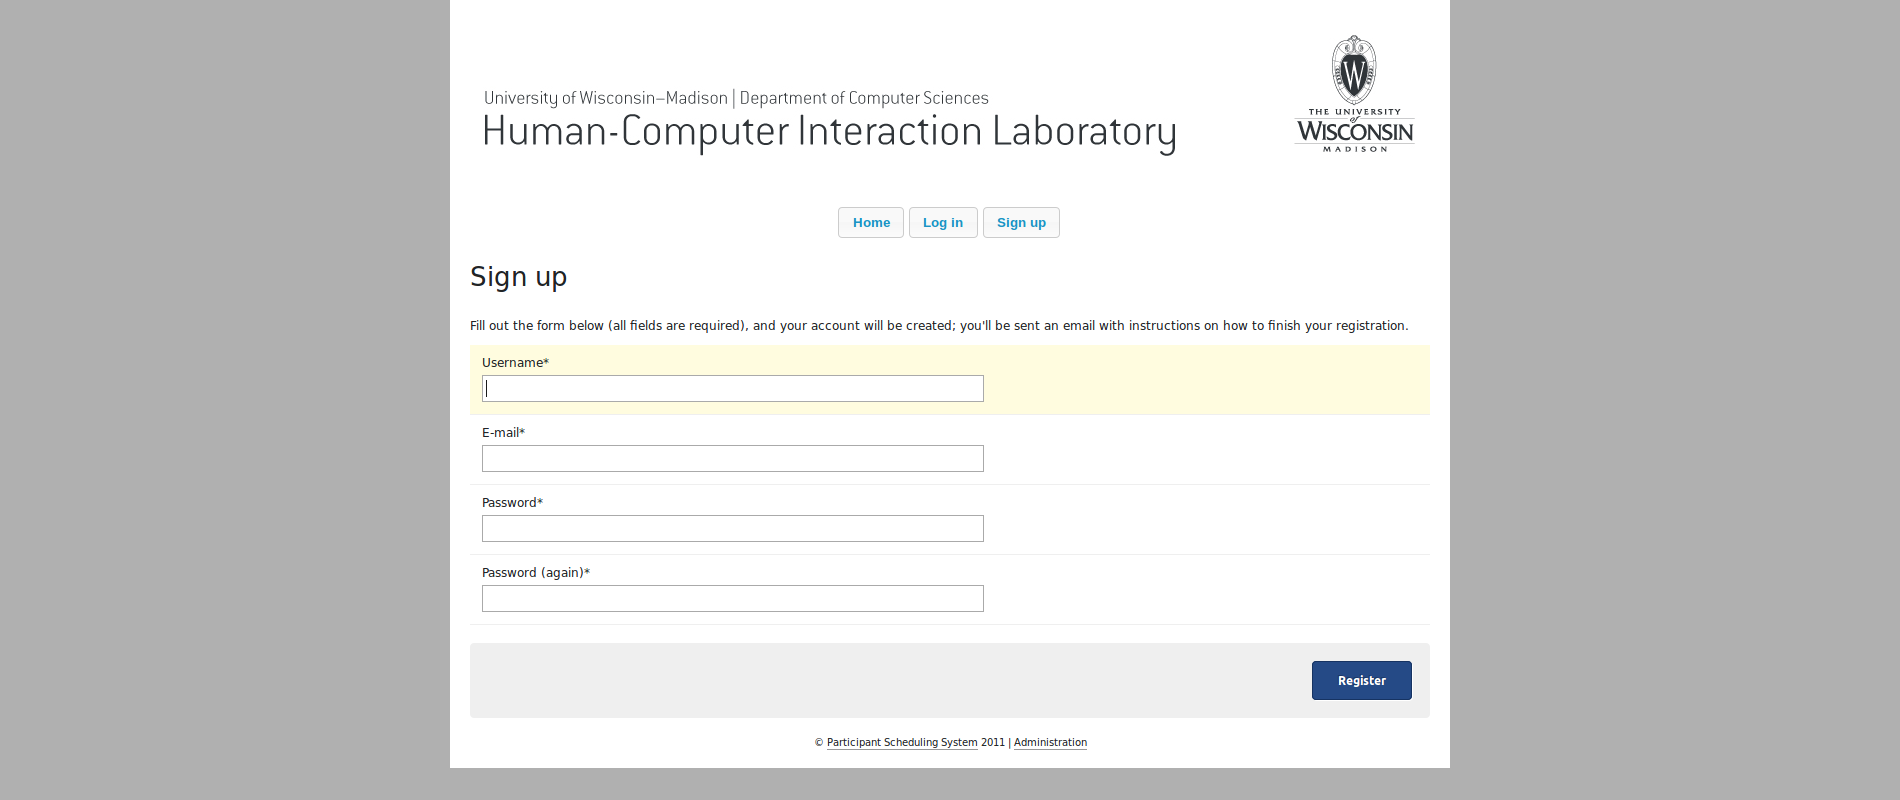
\includegraphics[width=6in]{../other/initial-interface-design/sign-up.png}
\subsubsection{Revised}
No changes

\subsection{Log In}
\subsubsection{Initial}
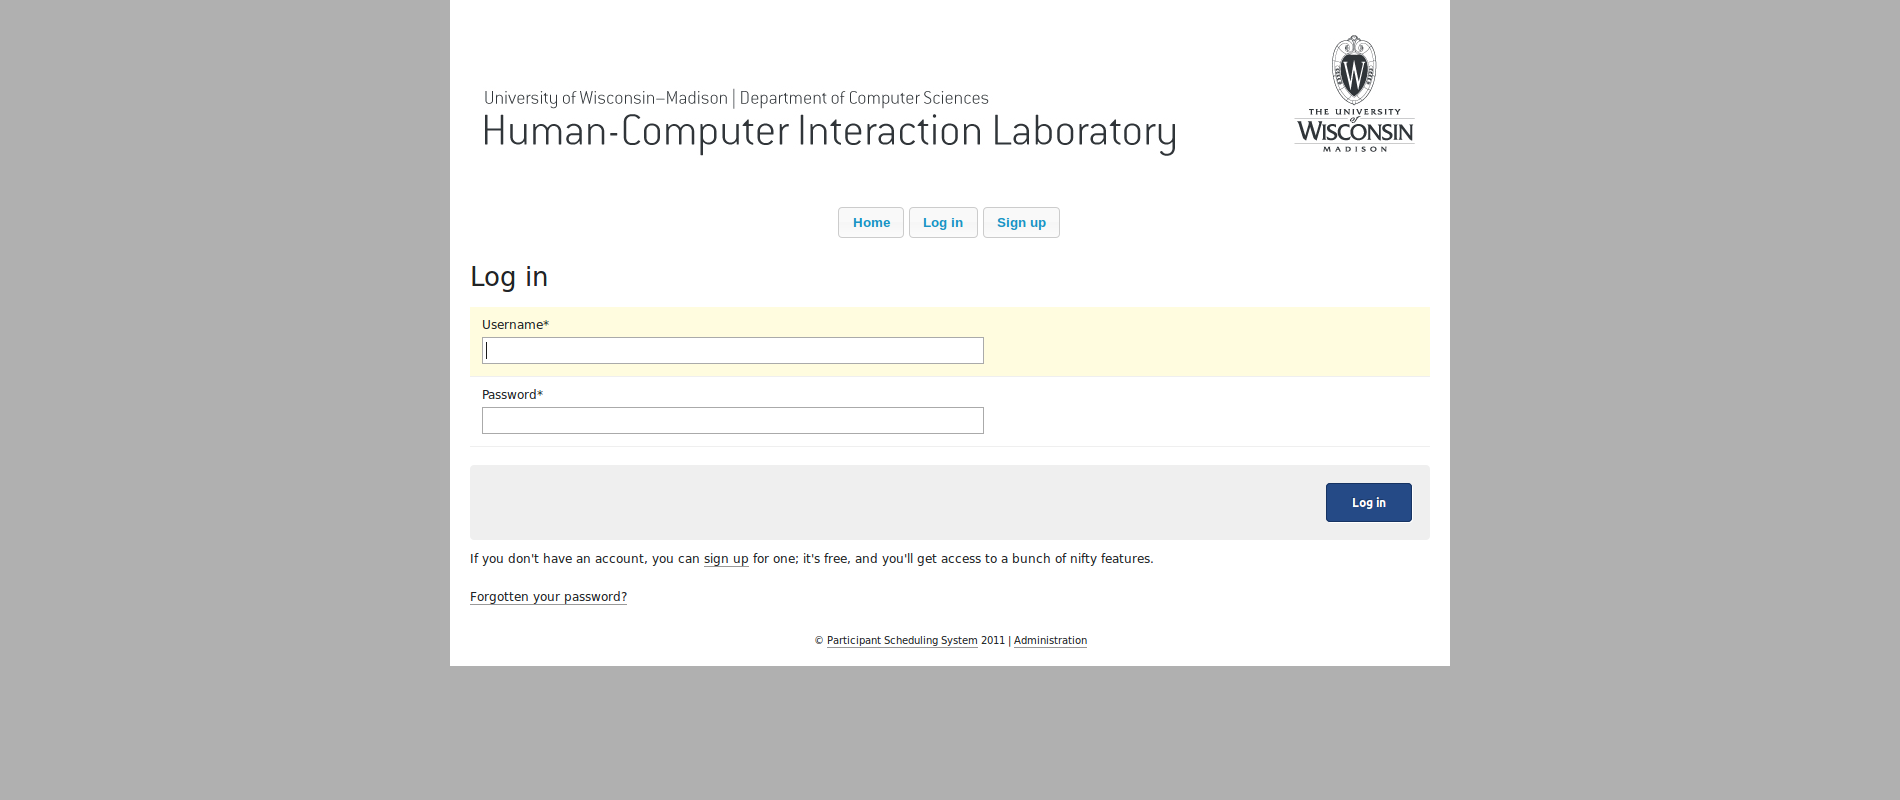
\includegraphics[width=6in]{../other/initial-interface-design/log-in.png}
\subsubsection{Revised}
No changes

\subsection{Password Reset}
\subsubsection{Initial}
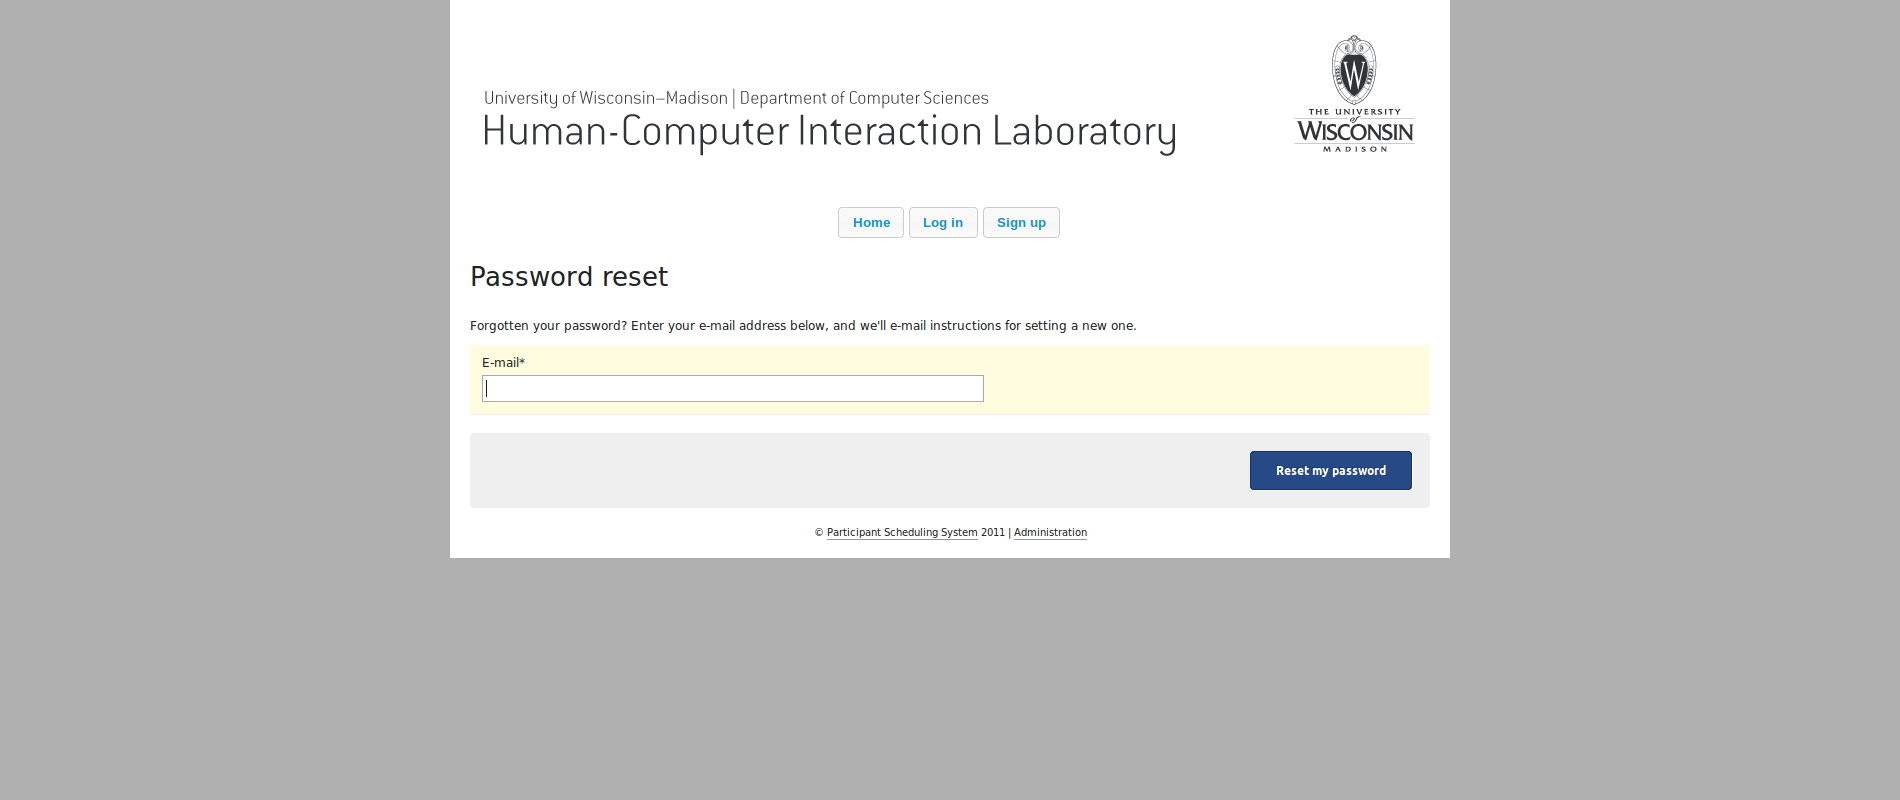
\includegraphics[width=6in]{../other/initial-interface-design/password-reset.png}
\subsubsection{Revised}
No changes

\subsection{Home, Logged In}
\subsubsection{Initial}

\includegraphics[width=6in]{../other/initial-interface-design/home-2.png}
\subsubsection{Revised}
Upon logging in, instead of being taken back to the home page, the user will be taken to the experiments page. If the user manually returns to the home page while logged in, the revisions of the default home page will be reflected there as well; see \textbf{Home, Logged In}. On every page, the logged in user's username or name will be displayed somewhere.

\subsection{Password Change}
\subsubsection{Initial}
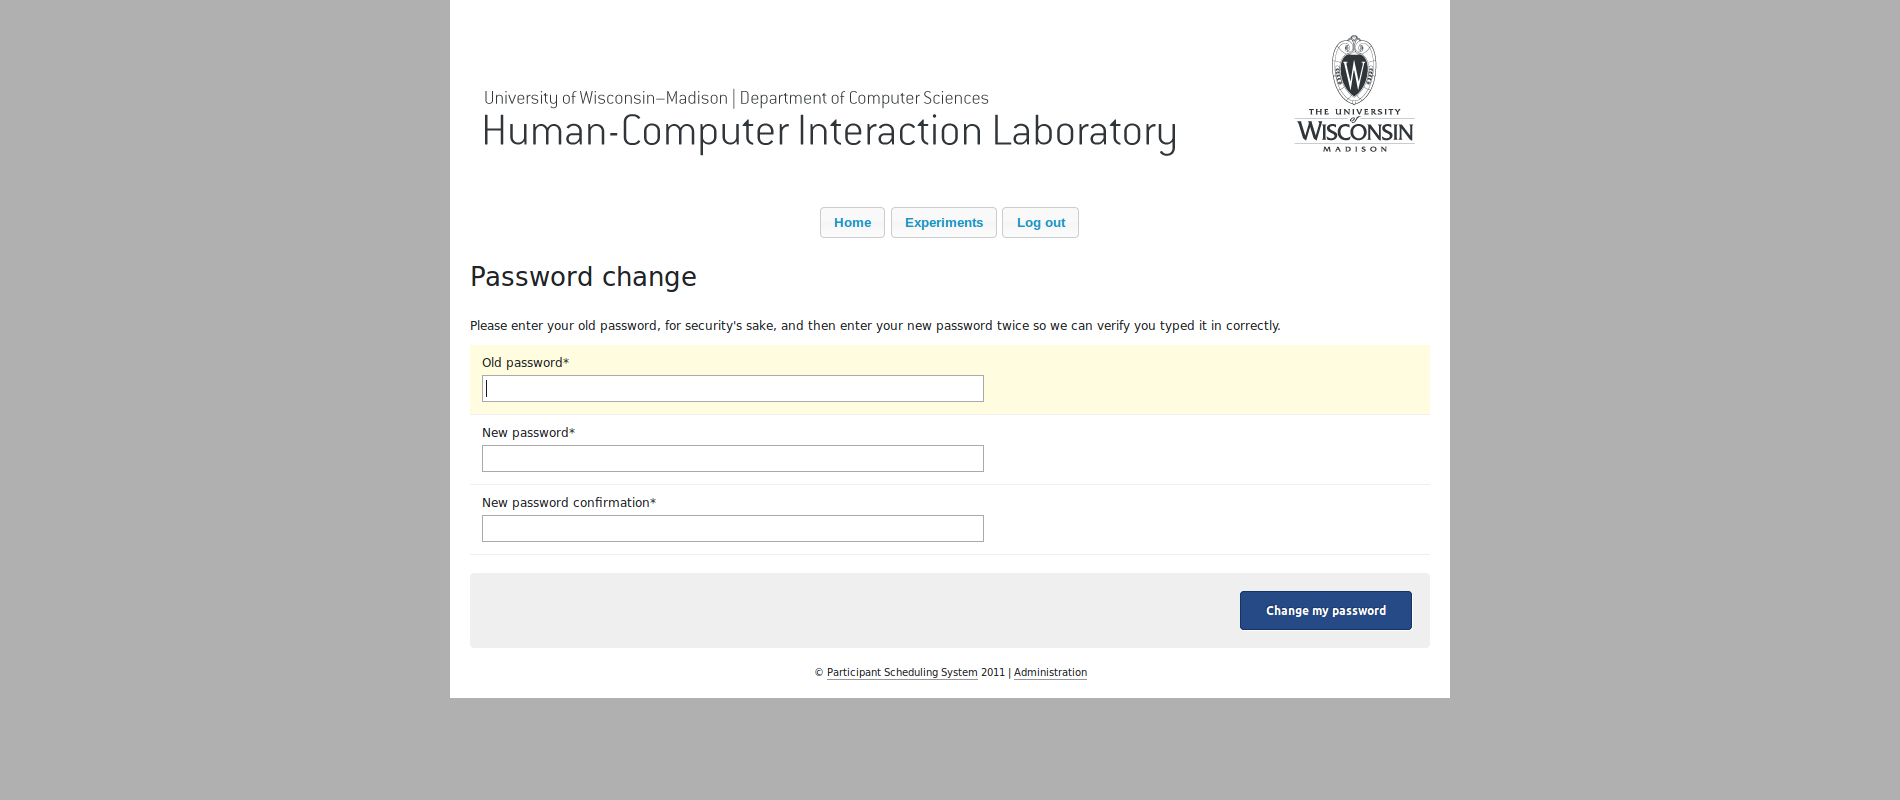
\includegraphics[width=6in]{../other/initial-interface-design/password-change.png}
\subsubsection{Revised}
It will be linked to from some other page, maybe the home page while logged in. No user was able to access it without explicitly visiting the URL, which they were not given.

\subsection{Experiments}
\subsubsection{Initial}
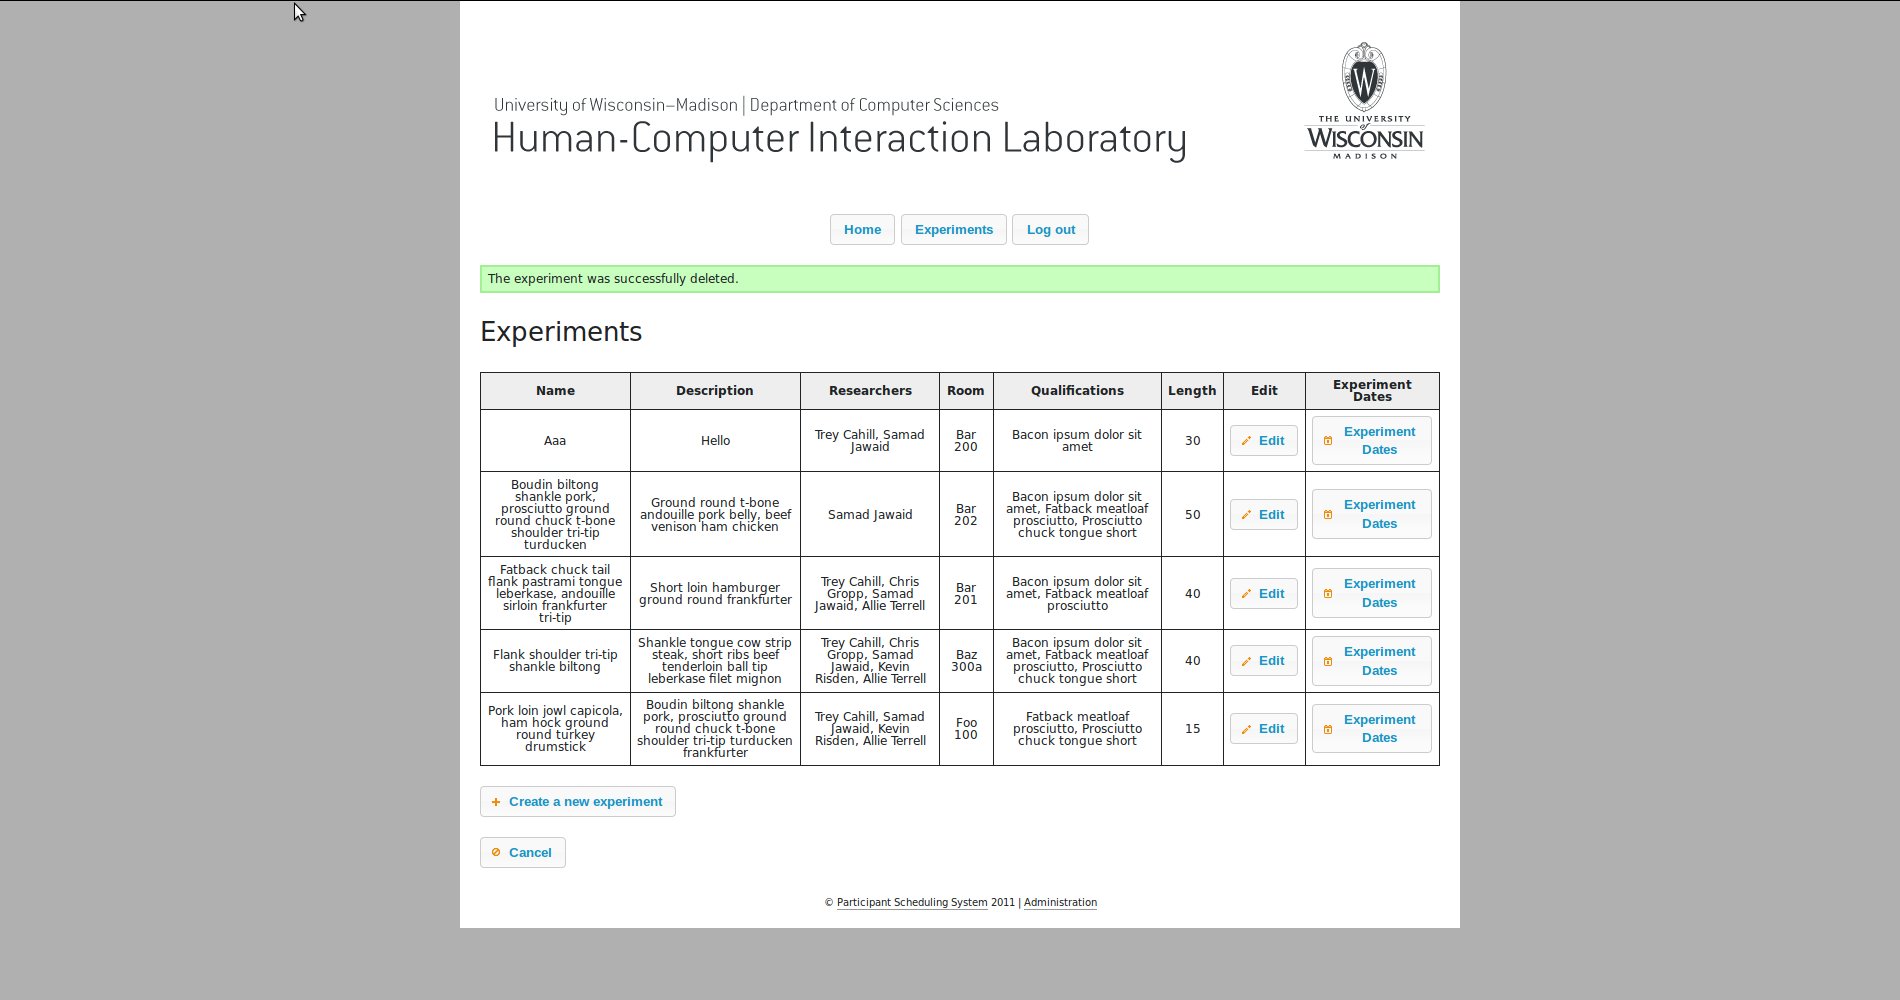
\includegraphics[width=6in]{../other/initial-interface-design/experiments.png}
\subsubsection{Revised}
The unit of length (minutes) will be specified. The table will be filterable and sortable. Experiments will be able to be mass-deleted from the table. The create button will be duplicated above the table as well. The cancel button will be changed to a back button with an appropriate icon.

\subsection{Create Experiment}
\subsubsection{Initial}
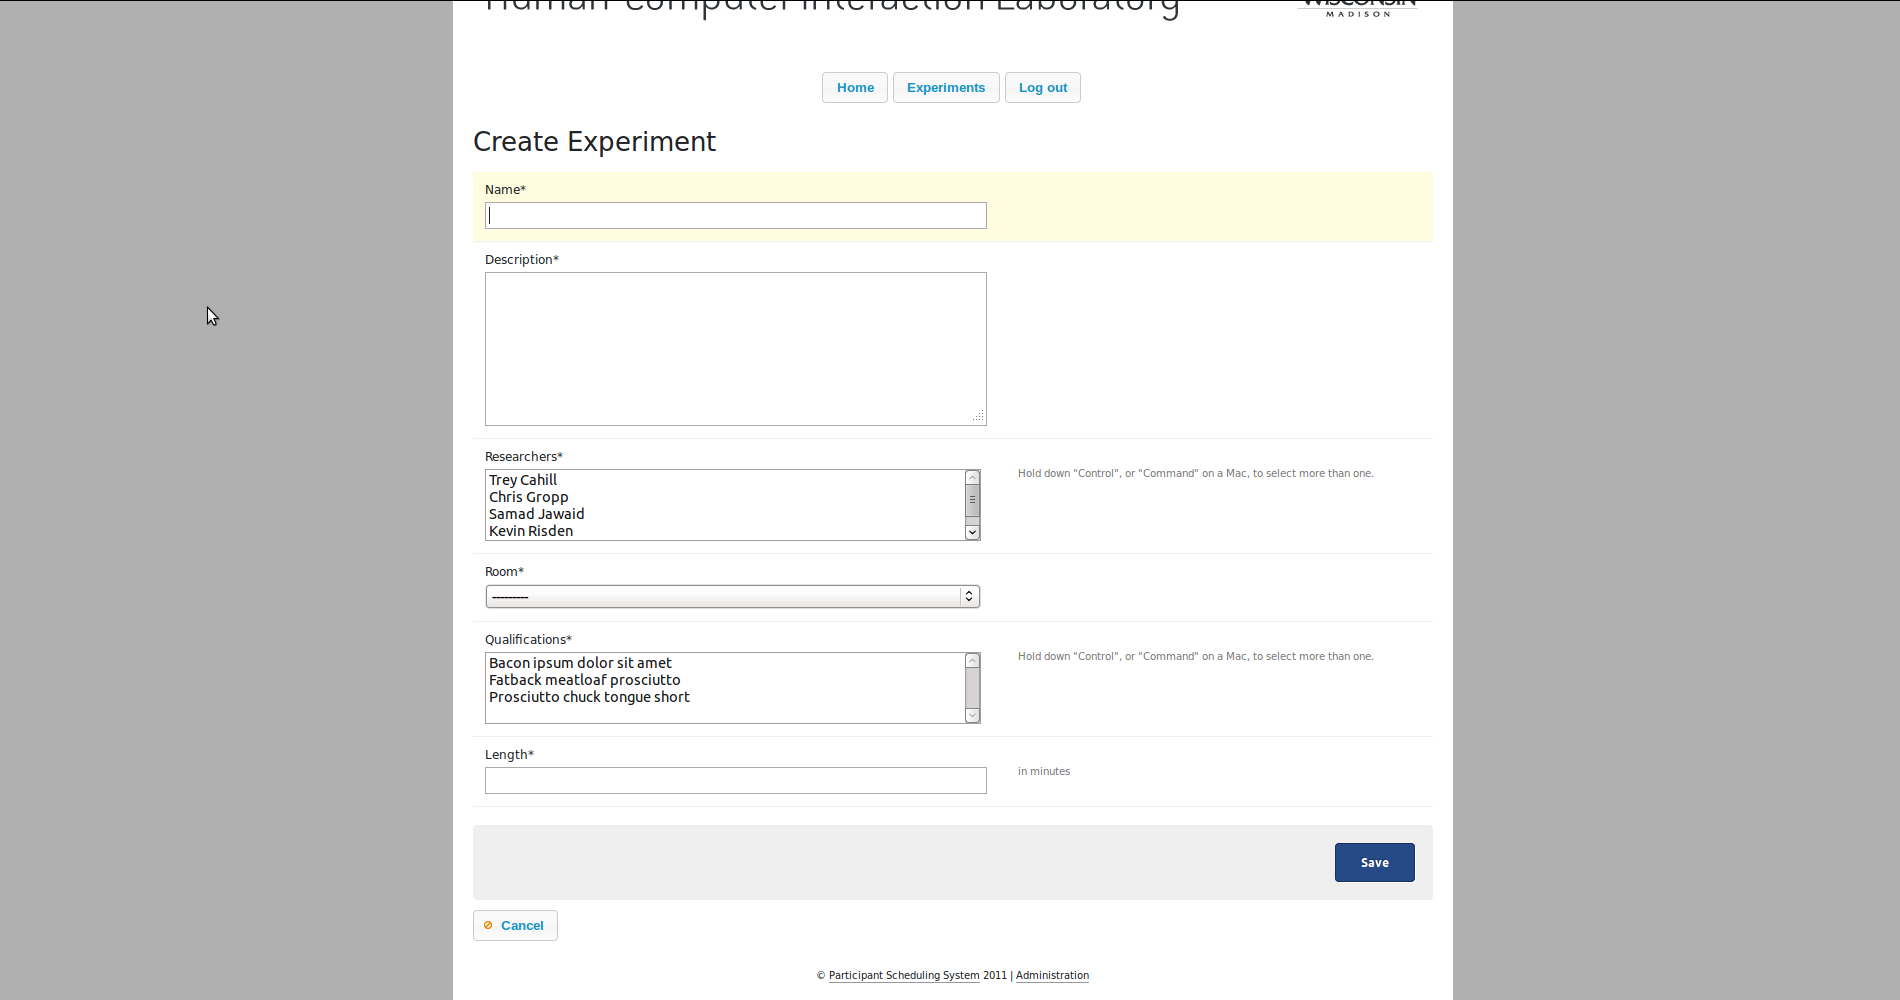
\includegraphics[width=6in]{../other/initial-interface-design/create-experiment.png}
\subsubsection{Revised}
The qualifications, room, and researchers inputs will be jQueryUI autocomplete fields with the ability to create new values. It will be clear that the cancel button discards all unsaved changes.

\subsection{Edit Experiment}
\subsubsection{Initial}
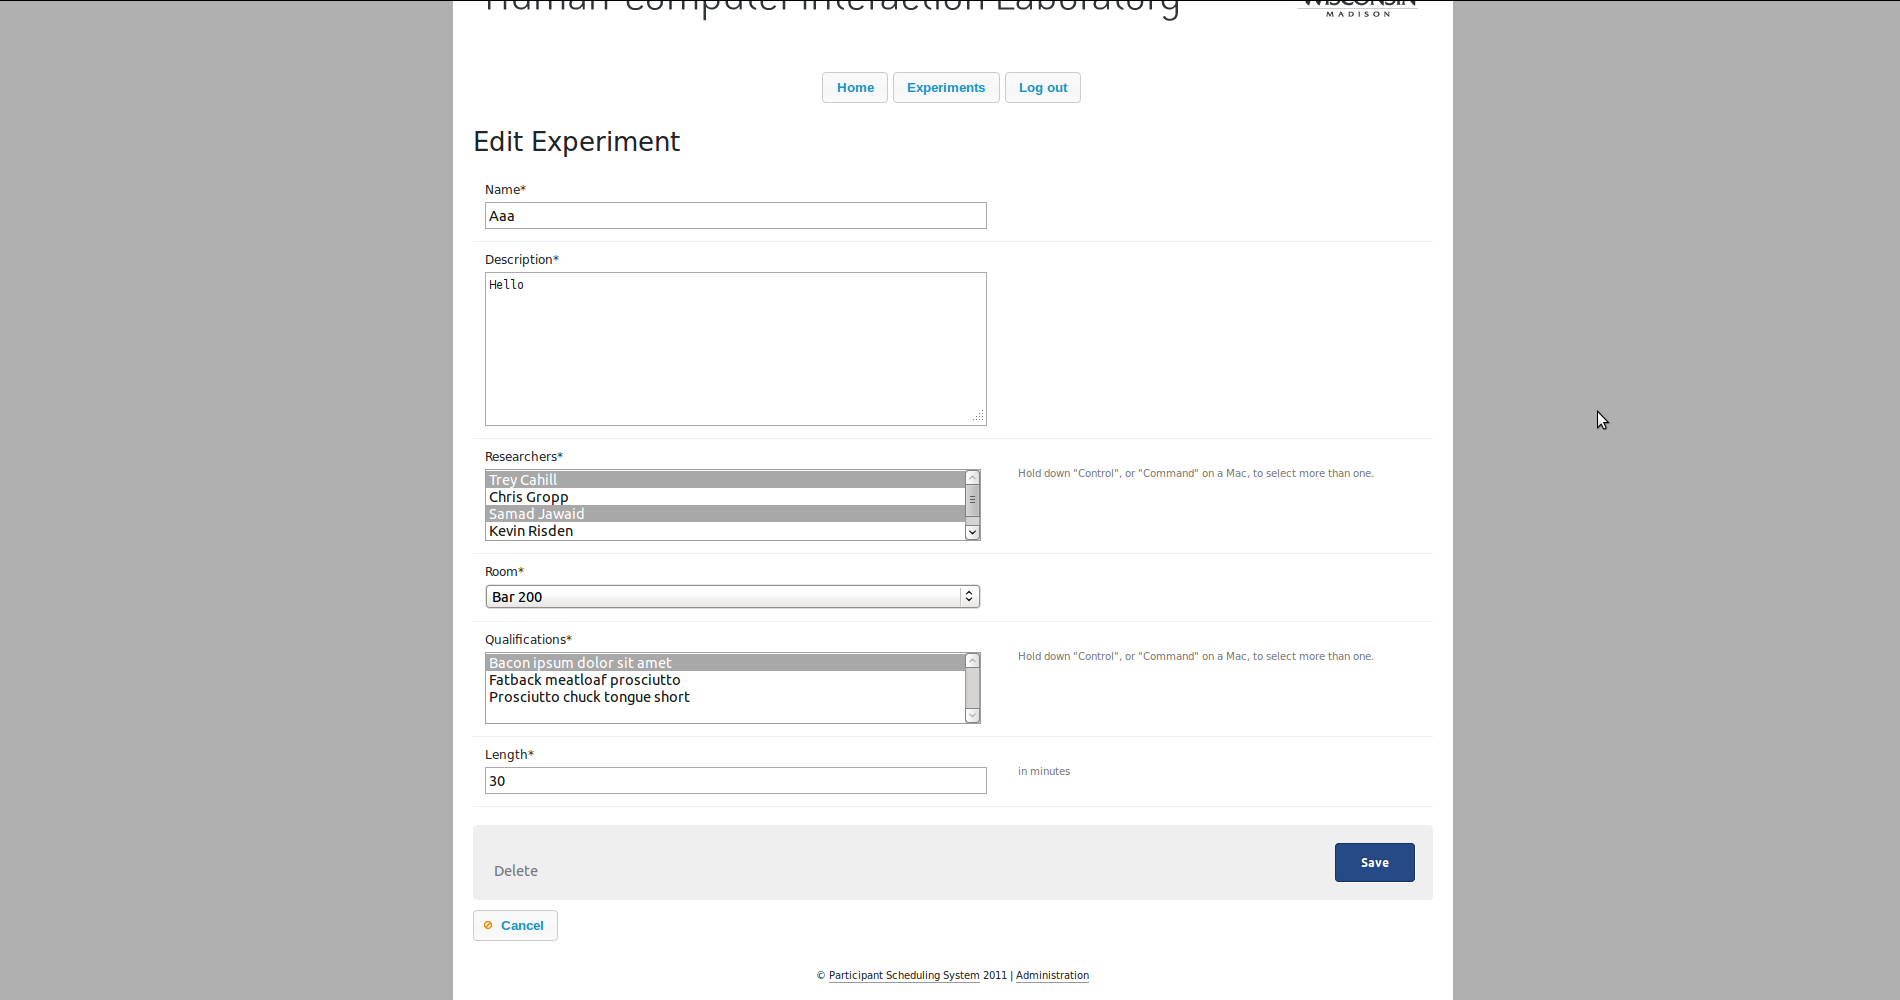
\includegraphics[width=6in]{../other/initial-interface-design/edit-experiment.png}
\subsubsection{Revised}
The delete button will not be so subtle. Also, see \textbf{Create Experiment}.

\subsection{Delete Experiment}
\subsubsection{Initial}
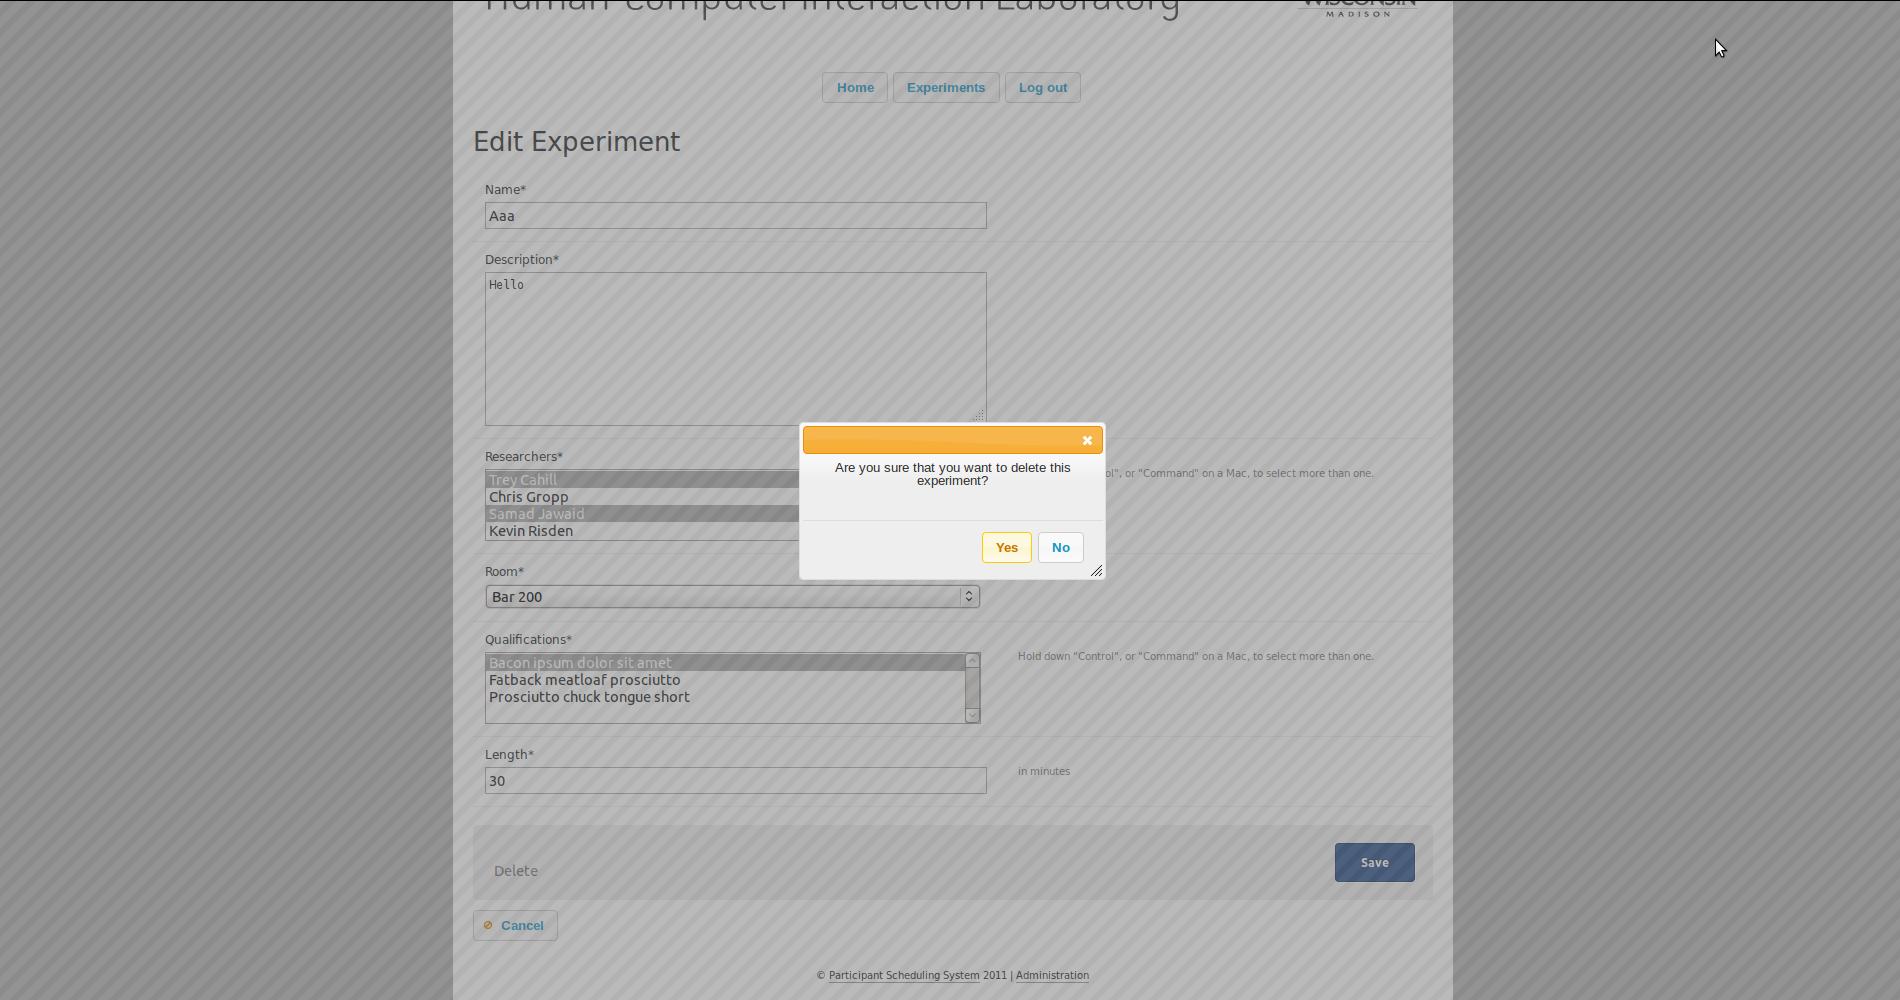
\includegraphics[width=6in]{../other/initial-interface-design/delete-experiment.png}
\subsubsection{Revised}
The jQueryUI CSS theme will match the existing CSS, so the dialog box will not appear so out of place.

\subsection{Experiment Dates}
\subsubsection{Initial}
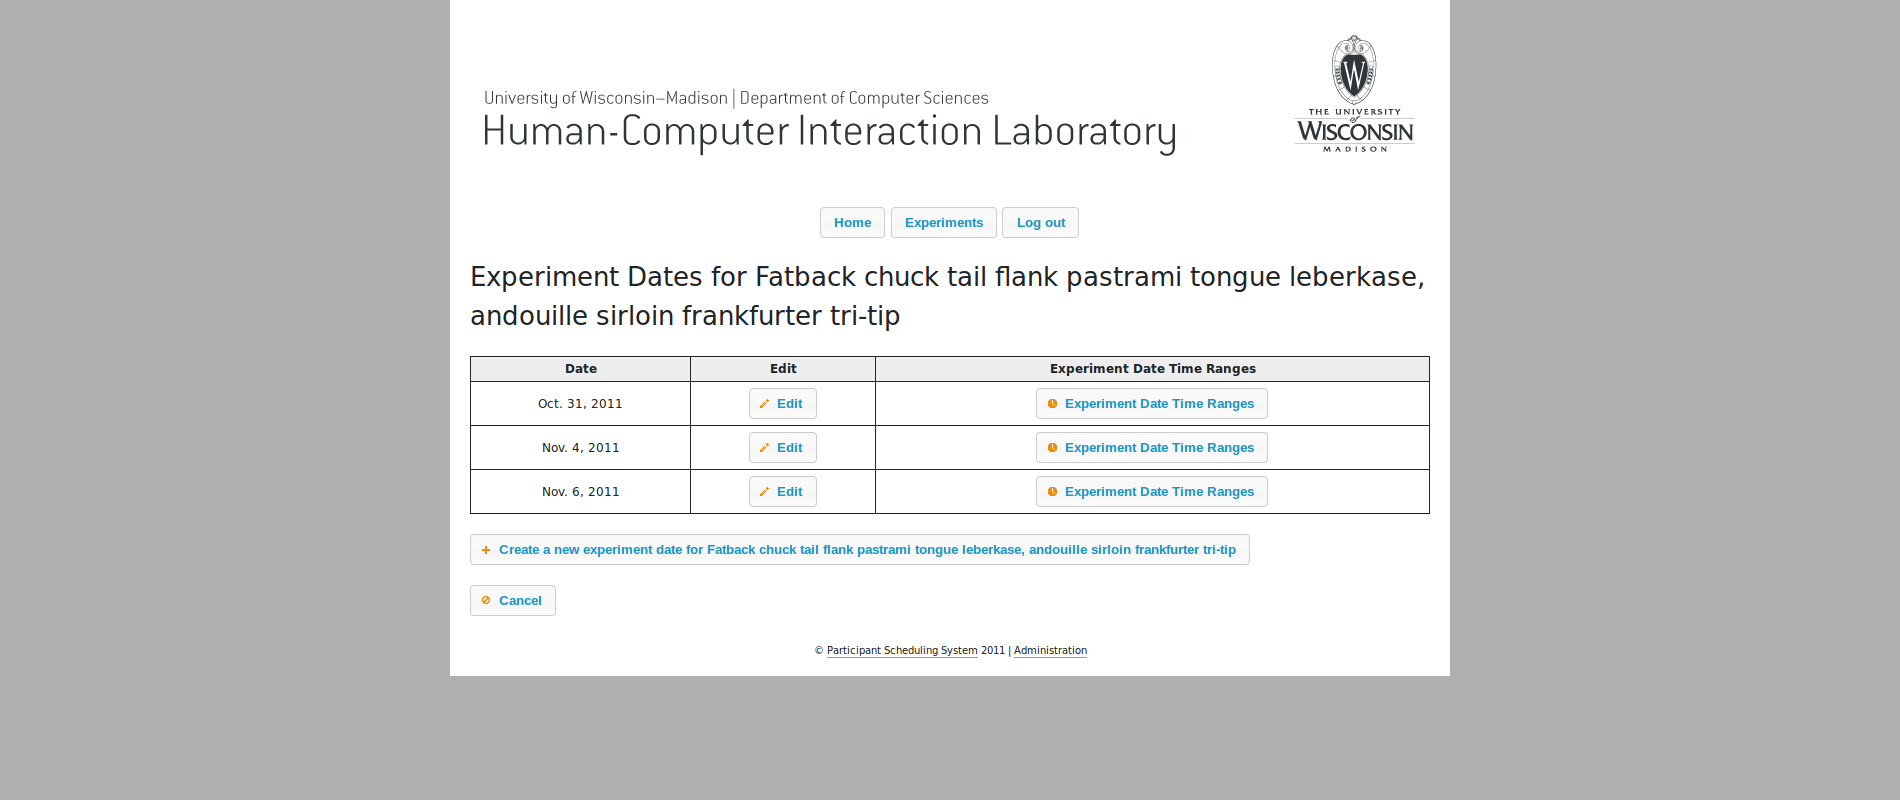
\includegraphics[width=6in]{../other/initial-interface-design/experiment-dates.png}
\subsubsection{Revised}
The table will be filterable and sortable. Experiment dates will be able to be mass-deleted from the table. The create button will be duplicated above the table as well. The cancel button will be changed to a back button with an appropriate icon.

\subsection{Create Experiment Date}
\subsubsection{Initial}
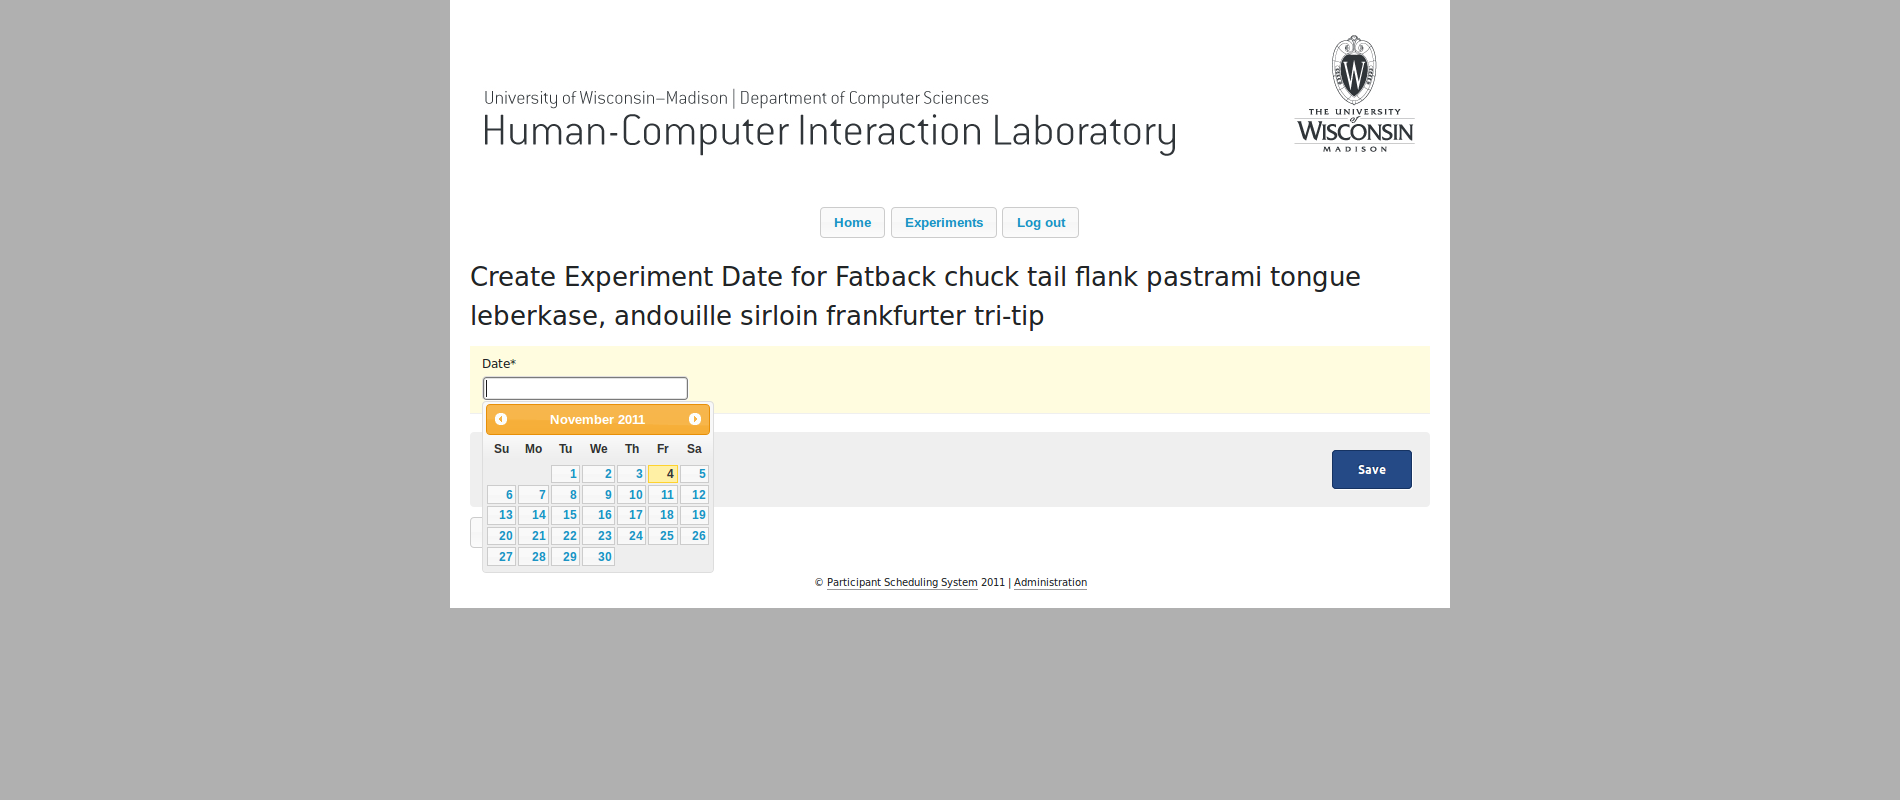
\includegraphics[width=6in]{../other/initial-interface-design/create-experiment-date.png}
\subsubsection{Revised}
The user will be able to type in a date manually without using the calendar widget. Help text explaining the date format will be added. The widget will not automatically appear on page load. It will be clear that the cancel button discards all unsaved changes.

\subsection{Edit Experiment Date}
\subsubsection{Initial}
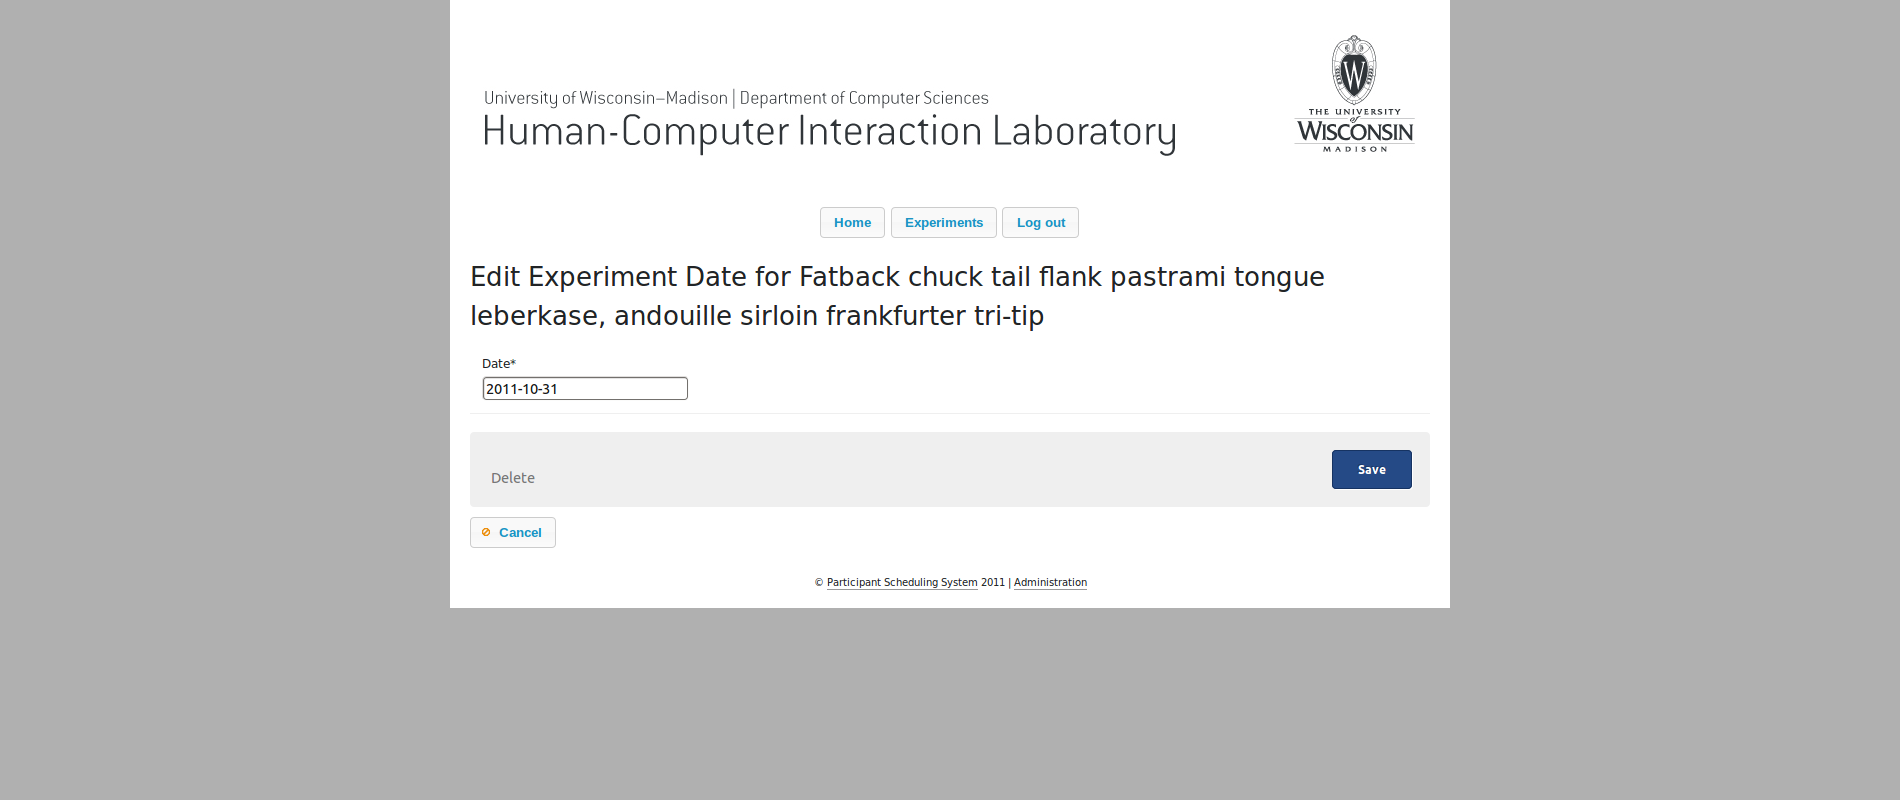
\includegraphics[width=6in]{../other/initial-interface-design/edit-experiment-date.png}
\subsubsection{Revised}
The delete button will not be so subtle. Also, see \textbf{Create Experiment Date}.

\subsection{Delete Experiment Date}
\subsubsection{Initial}
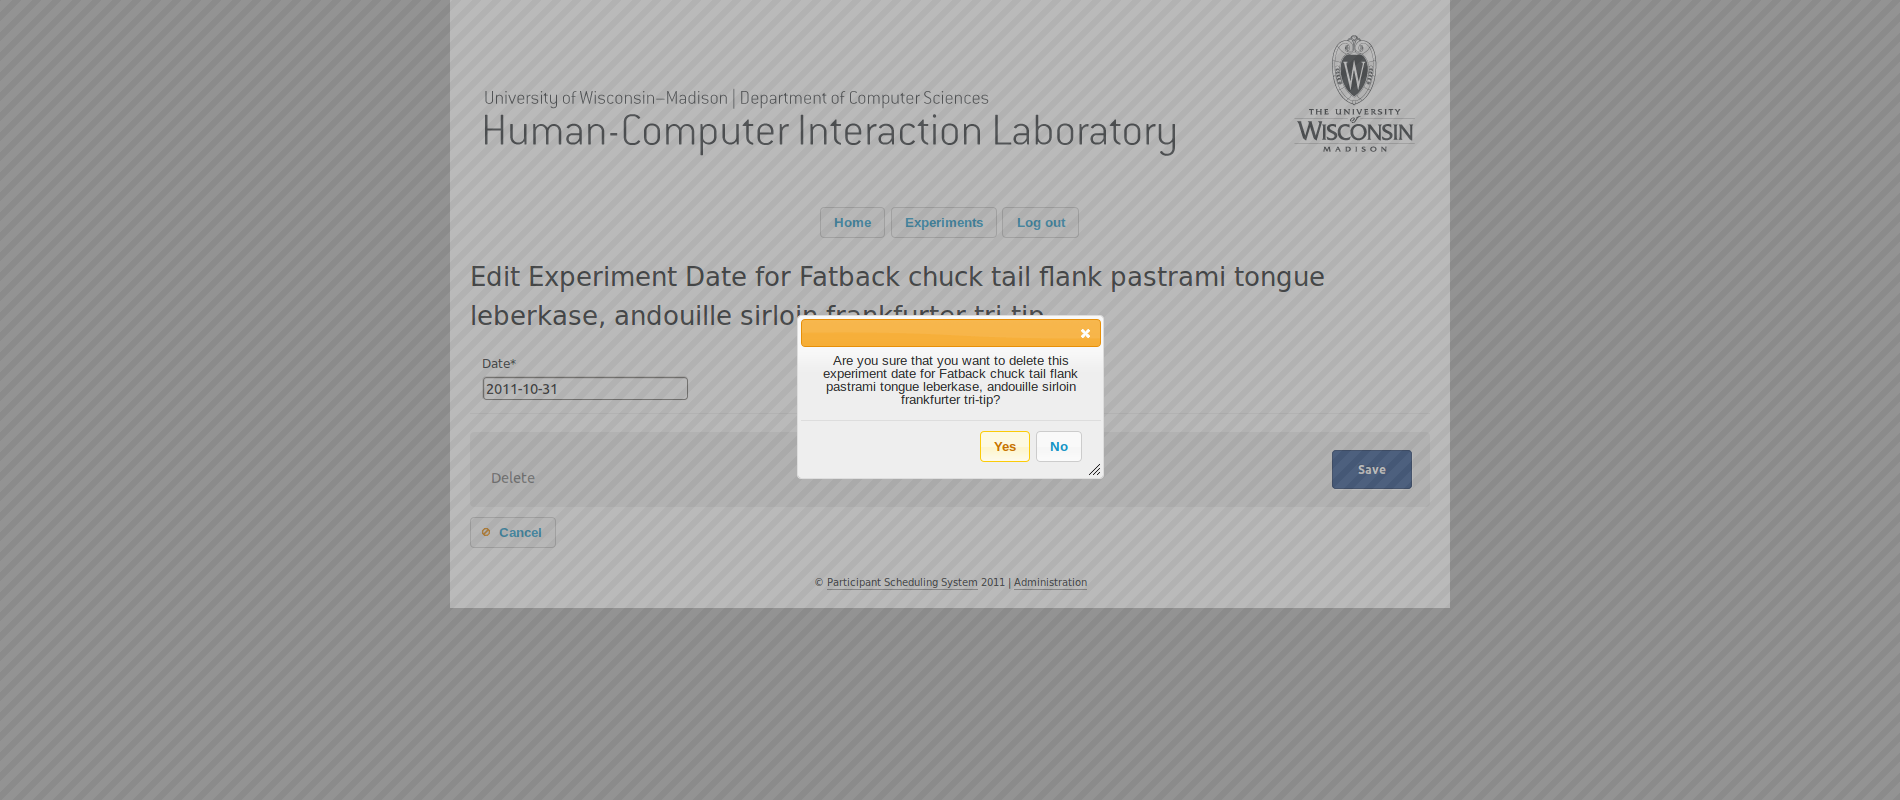
\includegraphics[width=6in]{../other/initial-interface-design/delete-experiment-date.png}
\subsubsection{Revised}
The jQueryUI CSS theme will match the existing CSS, so the dialog box will not appear so out of place.

\subsection{Experiment Date Time Ranges}
\subsubsection{Initial}
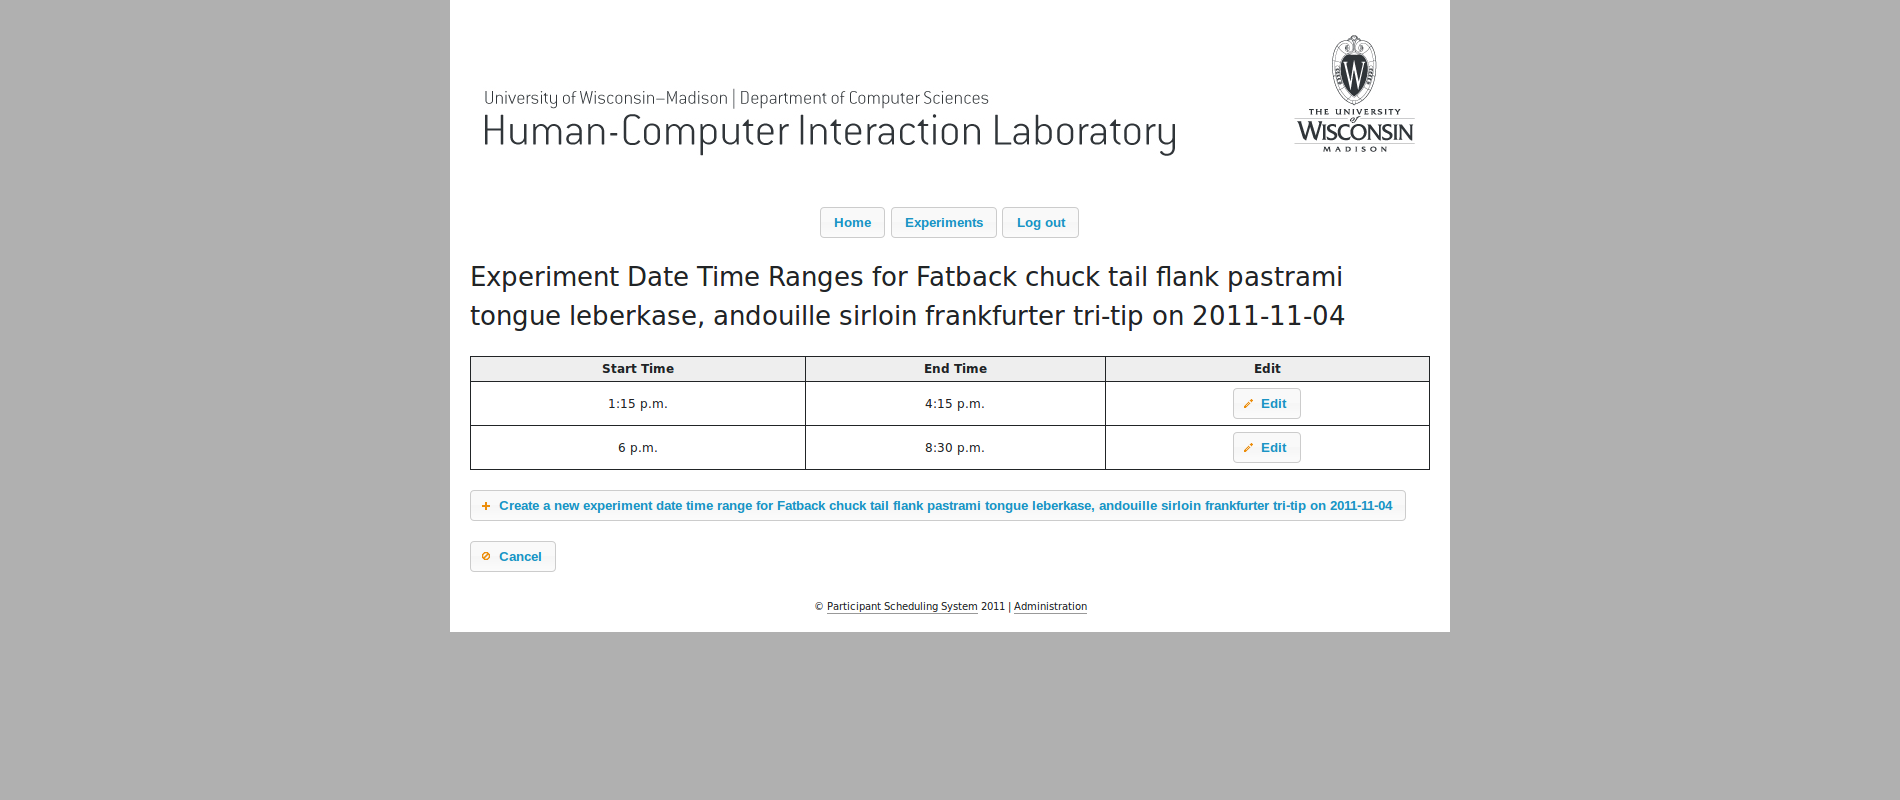
\includegraphics[width=6in]{../other/initial-interface-design/experiment-date-time-ranges.png}
\subsubsection{Revised}
The table will be filterable and sortable. Experiment date time ranges will be able to be mass-deleted from the table. The create button will be duplicated above the table as well. The cancel button will be changed to a back button with an appropriate icon.

\subsection{Create Experiment Date Time Range}
\subsubsection{Initial}
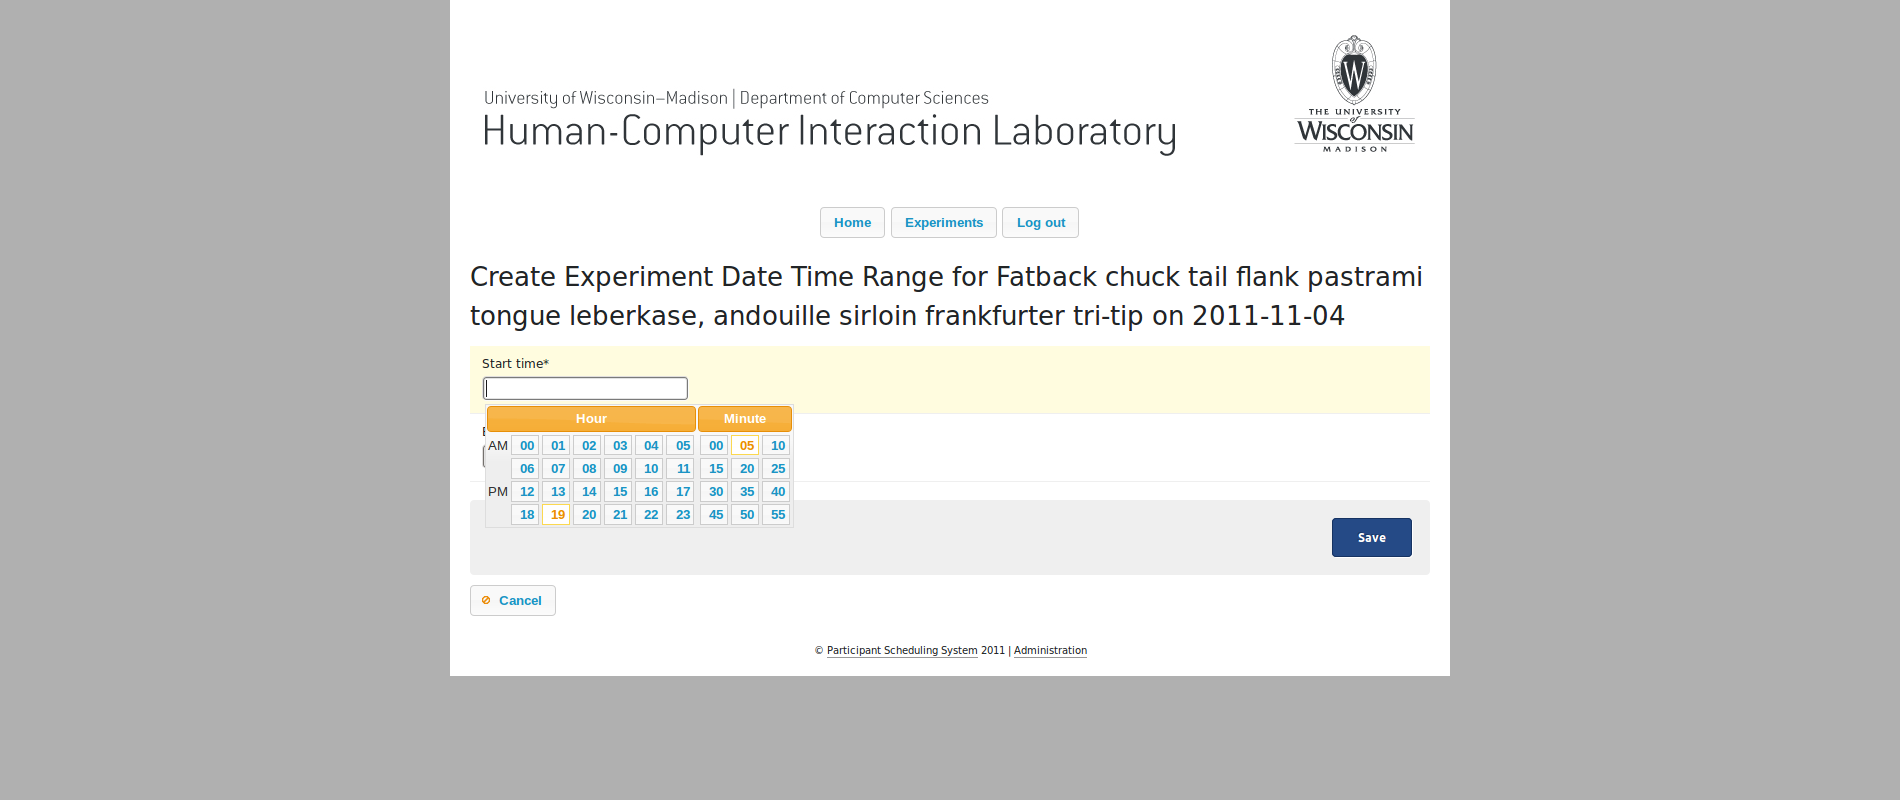
\includegraphics[width=6in]{../other/initial-interface-design/create-experiment-date-time-range.png}
\subsubsection{Revised}
The time widget will not have the AM or PM labels since it uses 24-hour time. Help text explaining the time format will be added. The widget will not automatically appear on page load. It will be clear that the cancel button discards all unsaved changes.

\subsection{Edit Experiment Date Time Range}
\subsubsection{Initial}
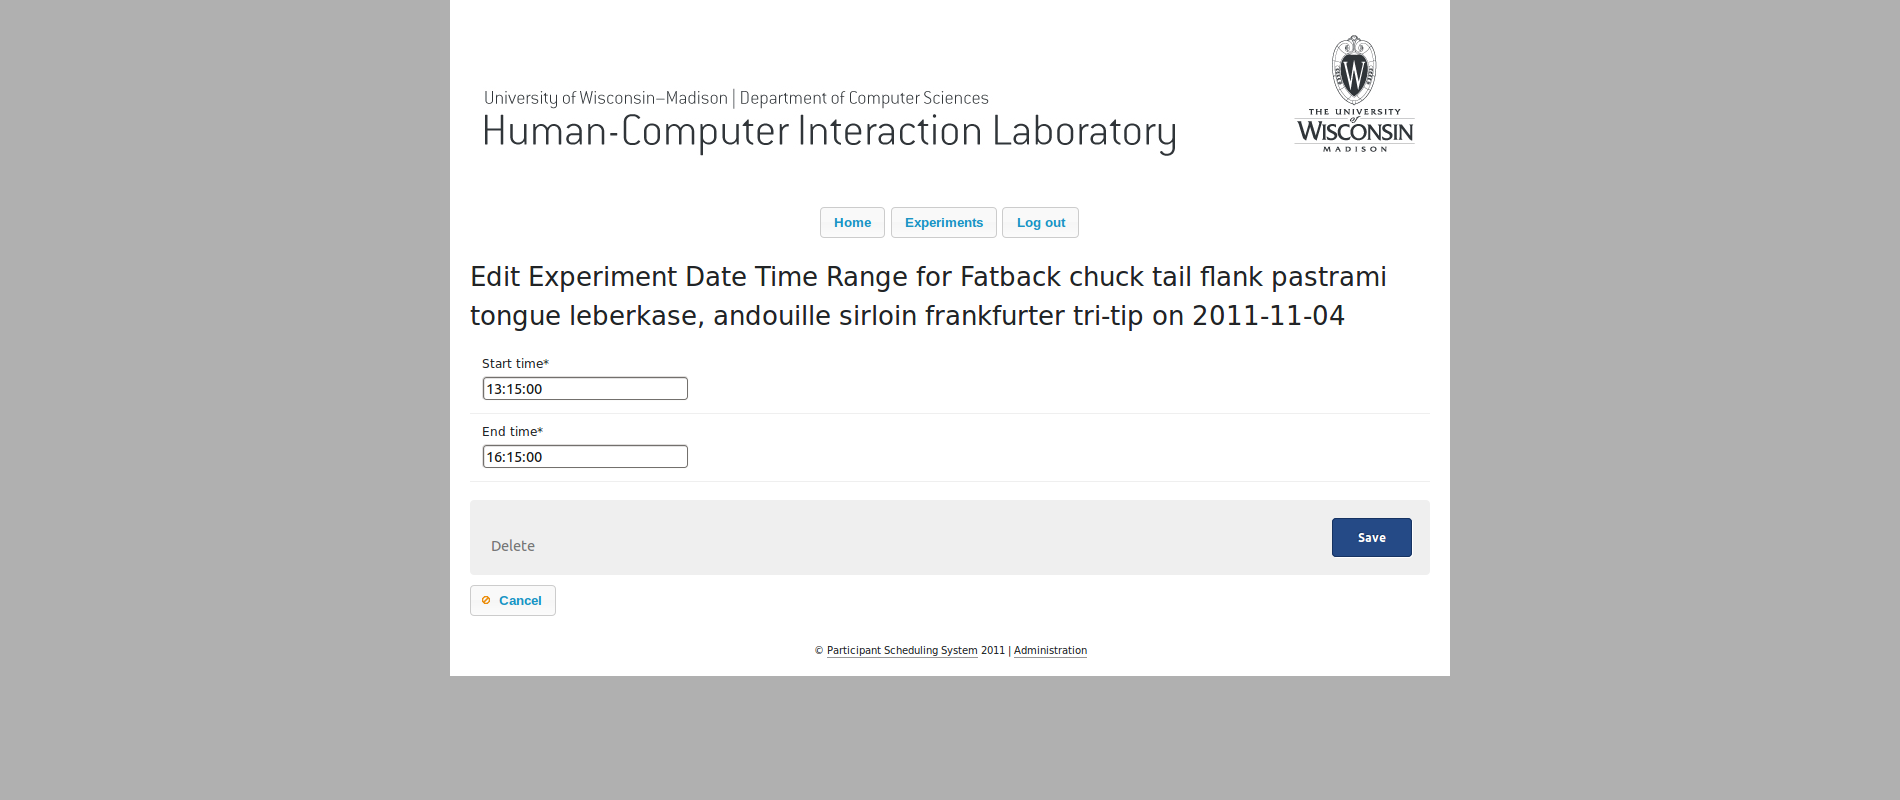
\includegraphics[width=6in]{../other/initial-interface-design/edit-experiment-date-time-range.png}
\subsubsection{Revised}
The delete button will not be so subtle. Also, see \textbf{Create Experiment Date Time Range}.

\subsection{Delete Experiment Date Time Range}
\subsubsection{Initial}
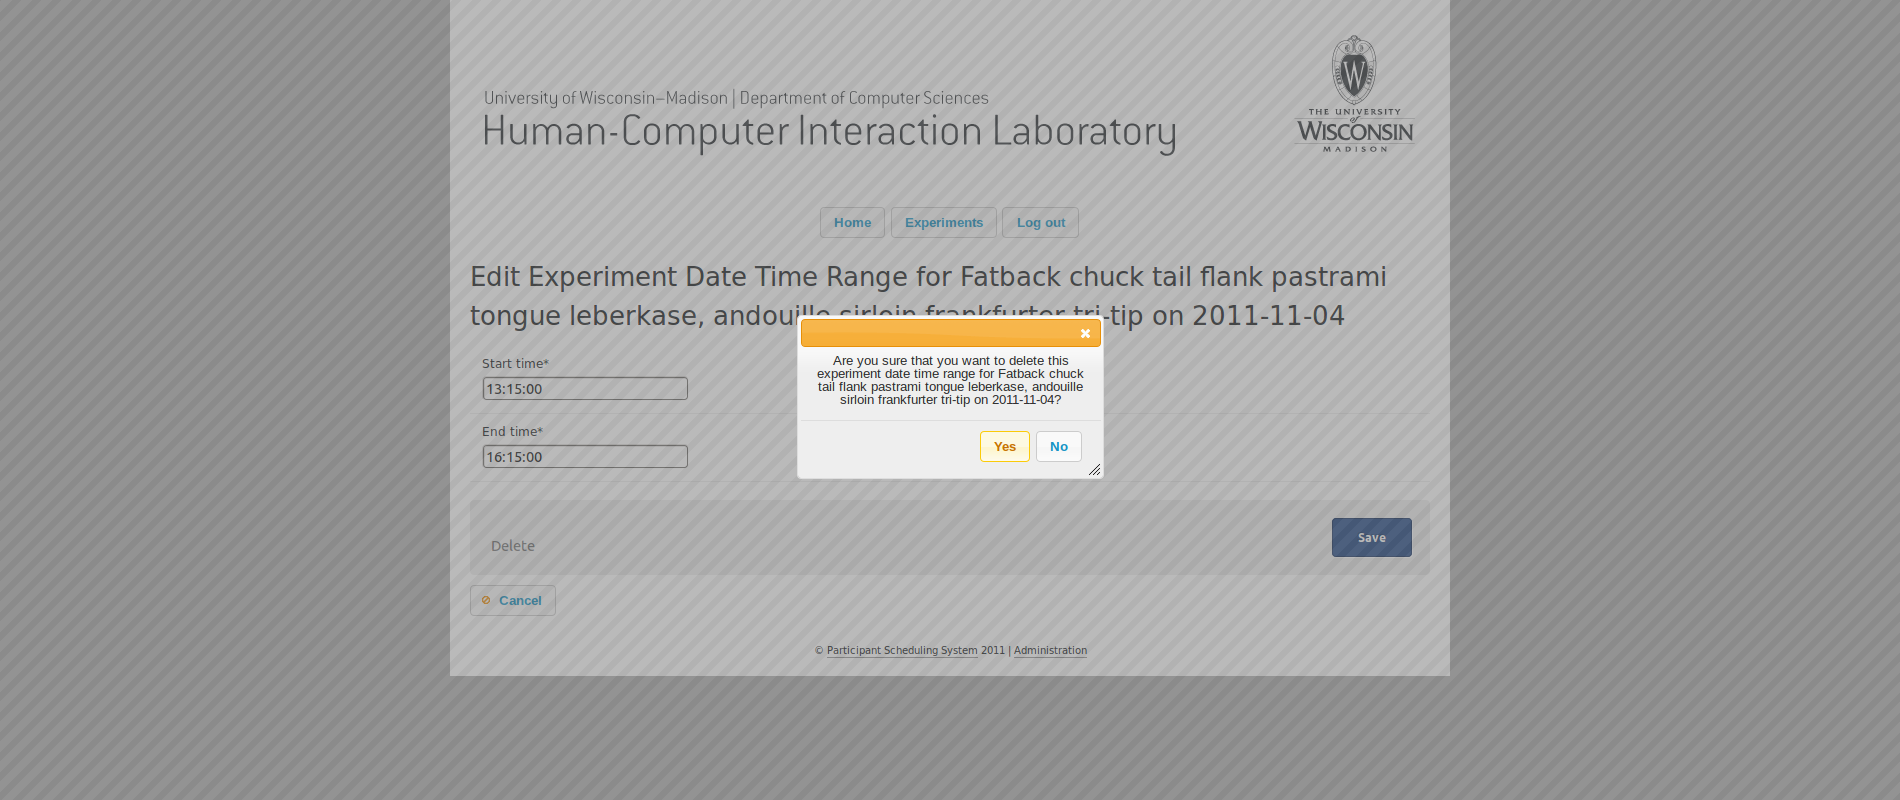
\includegraphics[width=6in]{../other/initial-interface-design/delete-experiment-date-time-range.png}
\subsubsection{Revised}
The jQueryUI CSS theme will match the existing CSS, so the dialog box will not appear so out of place.

% End - Milestone 5 specific parts
% fix for bibliography title
\renewcommand\refname{\section{References}}{\vspace*{-12mm}}
\bibliographystyle{plain}
\bibliography{bibliography}

\section{Appendix}

\section{Glossary}

\section{Index}

\end{document}
